\documentclass[12pt]{article}%
\usepackage{amsfonts}
\usepackage{fancyhdr}
\usepackage[hidelinks]{hyperref}
\usepackage[a4paper, top=2.5cm, bottom=2.5cm, left=2.2cm, right=2.2cm]%
{geometry}
\usepackage{times}
\usepackage{amsmath}
\usepackage{amsthm}
\usepackage{changepage}
\usepackage{amssymb}
\let\proof\relax
\let\endproof\relax
\usepackage{graphicx}%
\usepackage{qtree}
\usepackage{tikz}
\usetikzlibrary{positioning,automata}
\usepackage{adjustbox}
\usepackage{subcaption}
\setcounter{MaxMatrixCols}{30}
\newtheorem{theorem}{Theorem}
\newtheorem{corollary}[theorem]{Corollary}
\newtheorem{definition}[theorem]{Definition}
\newtheorem{lemma}[theorem]{Lemma}
\newtheorem{proposition}[theorem]{Proposition}
\newenvironment{proof}[1][Proof]{\textbf{#1.} }{\ \rule{0.5em}{0.5em}}

\begin{document}

\title{COS 445 - PSet 5, Problem 3} %Replace X with homework number, Y with problem number.
\author{Odysseus} %Write your name here
\date{\today}
\maketitle
\section*{Problem 3: Bigger Badder Braess’ Paradox}
We wish to show two networks $G_{\epsilon}$ and $G^{\prime}_{\epsilon}$, cost functions $c_{e}(\cdot)$ for each edge, and $\vec{r}$ where $r_{ab}$ units of traffic want to travel from $a$ to $b$ for all nodes $a, b$ such that all given conditions are met. We present the following networks:

\begin{figure}[h]
\centering
\begin{subfigure}[b]{0.4\linewidth}
\centering
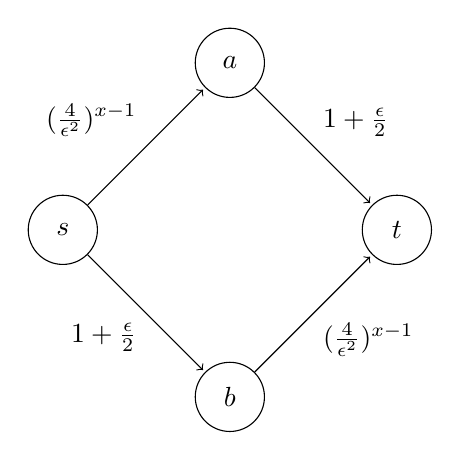
\begin{tikzpicture}[shorten >=1pt,node distance=3cm,on grid,auto]
  \node[state]  (0) 					{$s$};
  \node[state]  (1) [above right=of 0]		{$a$};
  \node[state]  (2) [below right=of 0]		{$b$};
  \node[state]  (3) [below right=of 1]		{$t$};
   \path[->]
   (0) edge node 	    {$(\frac{4}{\epsilon^2})^{x - 1}$} 	(1)
   	edge node [swap] {$1 + \frac{\epsilon}{2}$}  		(2)
   (1) edge node 	    {$1 + \frac{\epsilon}{2}$} 		(3)
   (2) edge node [swap] {$(\frac{4}{\epsilon^2})^{x - 1}$} 	(3);
\end{tikzpicture}
\caption{$G_{\epsilon}$}
\end{subfigure}
\begin{subfigure}[b]{0.4\linewidth}
\centering
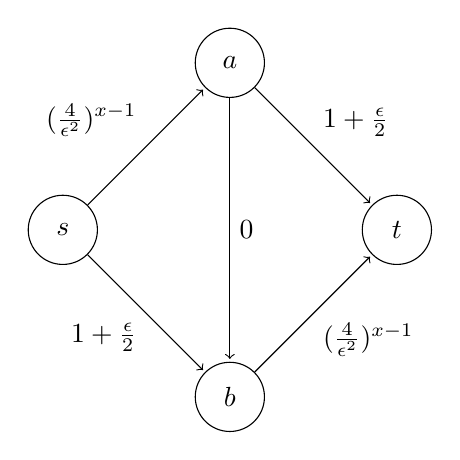
\begin{tikzpicture}[shorten >=1pt,node distance=3cm,on grid,auto]
  \node[state]  (0) 					{$s$};
  \node[state]  (1) [above right=of 0]		{$a$};
  \node[state]  (2) [below right=of 0]		{$b$};
  \node[state]  (3) [below right=of 1]		{$t$};
   \path[->]
   (0) edge node 	    {$(\frac{4}{\epsilon^2})^{x - 1}$} 	(1)
   	edge node [swap] {$1 + \frac{\epsilon}{2}$}  		(2)
   (1) edge node 	    {$1 + \frac{\epsilon}{2}$} 		(3)
   	edge node	    {$0$}						(2)
   (2) edge node [swap] {$(\frac{4}{\epsilon^2})^{x - 1}$} 	(3);
\end{tikzpicture}
\caption{$G^{\prime}_{\epsilon}$}
\end{subfigure}
\end{figure}

We note that the nodes in $G_{\epsilon}$ and $G^{\prime}_{\epsilon}$ are the same, that is they each contain the nodes $s$, $a$, $b$, and $t$. Additionally, all edges in $G_{\epsilon}$ are also present in $G^{\prime}_{\epsilon}$, with $G^{\prime}_{\epsilon}$ only having one additional edge between nodes $a$ and $b$. Each cost function on these edges is continuous, monotone non-decreasing, and non-negative.

We also observe that the unique equilibrium flow in $G_{\epsilon}$ has total cost at most $1 + \epsilon$. For example, if $\epsilon = \frac{1}{2}$ the resulting cost (no matter which direction is taken from $s$) is equal to $1 + \frac{\frac{1}{2}}{2} + (\frac{4}{(\frac{1}{2})^2})^{-\frac{1}{2}}$ or $1 + \frac{1}{2} = 1 + \epsilon$.

\end{document}
